%  ╦═╗┌─┐┌─┐┌─┐┌┐┌┌─┐┌─┐┬┌┬┐┬┌─┐┌┐┌┌┬┐┌─┐  ┌┬┐┌─┐  ┬┌┬┐┌─┐┌─┐┌─┐┌┐┌┌─┐┌─┐
%  ╠╦╝├┤ │  │ │││││ ││  │││││├┤ │││ │ │ │   ││├┤   ││││├─┤│ ┬├┤ │││├┤ └─┐
%  ╩╚═└─┘└─┘└─┘┘└┘└─┘└─┘┴┴ ┴┴└─┘┘└┘ ┴ └─┘  ─┴┘└─┘  ┴┴ ┴┴ ┴└─┘└─┘┘└┘└─┘└─┘

\chapter{Sistema de reconocimiento de imágenes para el valor de medición}
\label{ch:image_recognition}
En esta sección se discute el desarrollo del sistema de reconocimiento de caracteres que será empleado para adquirir automáticamente un valor de medición que sea indicado en la pantalla del sonómetro bajo calibración.
Primero se introduce un algoritmo general con los pasos de procesamiento y clasificación de las imágenes;
luego, se presenta el fundamento teórico de cada uno de esos pasos.
Finalmente, se muestran y discuten los resultados de procesamiento de imagen sobre una muestra de un dígito, como también los resultados del clasificador implementado.

\section*{Algoritmo de reconocimiento de caracteres}
De manera general, la solución propuesta, para el reconocimiento del valor de medición indicado en la pantalla del sonómetro, consta de varios pasos que se presentan en el siguiente algoritmo.

\begin{algorithm}[H]
    \caption{Algoritmo del sistema de reconocimiento de imágenes.}
    \label{alg:image_recongnition}
    \scriptsize
    \DontPrintSemicolon
    \SetKwData{image}{image} \SetKwData{images}{images} \SetKwData{training}{training} \SetKwData{features}{features} \SetKwInOut{Output}{output}
    \KwData{\images $\leftarrow$ \text{Imágenes de entrenamiento si va a entrenar o fotos de la pantalla si va reconocer.}}
    \Output{Clases estimadas.}
    \BlankLine
    \training $\leftarrow$ \emph{True} $|$ \emph{False}\;
    \ForEach{\image $\in$ \images}{
        \textbackslash\textbackslash Las operaciones sobre \image son realizadas \emph{in place}.\;
        \textbf{\hyperref[sec:gaussian_filter]{Paso 1}:} Filtrar \image con filtro gaussiano.\;
        \textbf{\hyperref[sec:padding]{Paso 2}:} Escalar y hacer \emph{padding} a \image para hacerla de $31 \times 32$ píxeles.\;
        \textbf{\hyperref[sec:segmentation]{Paso 3}:} Segmentar \image determinando el umbral con el método de \citet{Otsu1979}.\;
        \If{\training $=$ False}{
            Detectar contornos y extraer dígitos.\;
        }
        \textbf{\hyperref[sec:sift_descriptor]{Paso 4}:} Calcular las características de \image con el descriptor SIFT~\citep{Lowe2004}.\;
        \textbf{\hyperref[sec:kpca_reduction]{Paso 5}:} Reducir dimensionalidad de las características por KPCA~\citep{Scholkopf1997}.\;
        Agregar las características a la matriz \features.\;
    }
    \textbf{\hyperref[sec:nb_classifier]{Paso 6}:}\;
    \eIf{\training}{
        Entrenar clasificador bayesiano normal con \features y las correspondientes etiquetas de clase.\;}
    {
        Estimar las clases de las características en \features con el clasificador bayesiano normal.\;}
\end{algorithm}

%\begin{figure}
%	\caption{Diagrama de flujo del algoritmo de reconocimiento de caracteres}
%	\label{fig:flowchart}
%	\centering
%	\begin{tikzpicture}[font=\scriptsize, node distance=1.5cm]
%		\node (start1) at (-6, 5) [draw, terminal, minimum width=2cm, minimum height=0.5cm] {Inicio};
%		\node (subrutine1) [draw, predproc, minimum width=2cm, align=center,
%							minimum height=0.5cm, below of=start1] {Entrenar \\ clasificador};
%		\node (process1) [draw, process, minimum width=2cm, align=center,
%						  minimum height=0.5cm, below of=subrutine1] {Configurar \\ multímetro};
%		\node (subrutine2) [draw, predproc, minimum width=2cm, align=center,
%							minimum height=0.5cm, below of=process1] {Detección del \\ área de interés (ROI)};
%		\node (process2) [draw, process, minimum width=2cm, align=center,
%						  minimum height=0.5cm, below of=subrutine2] {Enviar señal \\ de prueba};
%		\node (process2_north) [draw, circle, fill=black, inner sep=0pt,
%								minimum size=2pt, above of=process2, node distance=0.75cm] {};
%		\node (subrutine3) [draw, predproc, minimum width=2cm, align=center,
%							minimum height=0.5cm, below of=process2] {Reconocimiento \\ del resultado};
%		\node (storage1) [draw, storage, minimum width=2cm, align=center,
%						  minimum height=0.5cm, below of=subrutine3] {Almacenar \\ resultado};
%		\node (decide1) [draw, conditional, minimum width=2cm,
%						 minimum height=0.5cm, below of=storage1] {¿Prueba finalizada?};
%		\node (decide1_east) [right of=decide1, node distance=3cm]{};
%		\node (print1) [draw, print, minimum width=2cm, align=center,
%						minimum height=0.5cm, below of=decide1] {Presentar \\ resultados};
%		\node (finish1) [draw, terminal, minimum width=2cm, minimum height=0.5cm, below of=print1] {Fin};
%
%		\draw [arrow] (start1) -- (subrutine1);
%		\draw [arrow] (subrutine1) -- (process1);
%		\draw [arrow] (process1) -- (subrutine2);
%		\draw [arrow] (subrutine2) -- (process2);
%		\draw [arrow] (process2) -- (subrutine3);
%		\draw [arrow] (subrutine3) -- (storage1);
%		\draw [arrow] (storage1) -- (decide1);
%		\draw [thick] (decide1) -- node[pos=0.1, above]{No} (decide1_east.center);
%		\draw [arrow] (decide1_east.center) |- (process2_north);
%		\draw [arrow] (decide1) -- node[right] {Sí} (print1);
%		\draw [arrow] (print1) -- (finish1);
%		
%		\node (start2) at (0, 5) [draw, terminal, minimum width=2cm,
%								  align=center, minimum height=0.5cm] {Entrenar \\ clasificador};
%		\node (process3) [draw, process, minimum width=2cm, minimum height=0.5cm,
%						  align=center, below of=start2] {Filtro \\ gaussiano};
%		\node (database1) [minimum width=2cm, right of=start2,
%						  node distance = 3 cm, align=center] {Imágenes de \\ entrenamiento};
%		\draw (database1.north west) -- (database1.south west)
%			  .. controls +(-30:0.2cm) and +(-150:0.2cm) .. (database1.south east)
%			  -- (database1.north east) .. controls +(-150:0.2cm) and +(-30: 0.2cm) .. (database1.north west)
%			  -- +(0, 0.2cm) .. controls +(-30:0.2cm) and +(-150:0.2cm) .. +(2.01cm, 0.2cm)
%			  .. controls +(150:0.2cm) and +(30:0.2cm) .. +(0,0.2cm) -- +(0, 0.1cm)
%			  .. controls +(-30:0.2cm) and +(-150:0.2cm) .. +(2.01cm, 0.1cm)
%			  -- (database1.north east) -- +(0cm, 0.2cm);
%		\node (process4) [draw, process, minimum width=2cm, align=center,
%						  minimum height=0.5cm, below of=process3] {Escalización \\ y \emph{padding}};
%		\node (process5) [draw, process, minimum width=2cm, minimum height=0.5cm, below of=process4] {Binarización};
%		\node (process6) [draw, process, minimum width=2cm, align=center,
%						  minimum height=0.5cm, below of=process5] {Cálculo del \\ descriptor SIFT};
%		\node (process7) [draw, process, minimum width=2cm, align=center,
%						  minimum height=0.5cm, below of=process6] {Reducción de \\ dimensionalidad con \\ KPCA};
%		\node (process8) [draw, process, minimum width=2cm, align=center,
%						  minimum height=0.5cm, below of=process7] {Ajuste del clasificador \\ normal bayessiano};
%		\node (finish2) [draw, terminal, minimum width=2cm, minimum height=0.5cm, below of=process8] {Volver};
%		
%		\draw [arrow] (start2) -- (process3);
%		\draw [thick, <-, stealth-] (process3.east) -| ++(2cm, 1.08cm);
%		\draw [arrow] (process3) -- (process4);
%		\draw [arrow] (process4) -- (process5);
%		\draw [arrow] (process5) -- (process6);
%		\draw [arrow] (process6) -- (process7);
%		\draw [arrow] (process7) -- (process8);
%		\draw [arrow] (process8) -- (finish2);
%		
%		\node (start3) at (7, 5) [draw, terminal, align=center,
%		minimum width=2cm, minimum height=0.5cm] {Reconocimiento \\ del resultado};
%		\node (process9) [draw, process, align=center, below of=start3,
%		            minimum width=2cm, minimum height=0.5cm,
%		            node distance=1.2cm] {Capturar imagen y \\ extraer región de interés};
%	    \node (process10) [draw, process, below of=process9, minimum width=2cm,
%	    				   minimum height=0.5cm, node distance=1.2cm] {Filtro gaussiano};
%	    \node (process11) [draw, process, below of=process10, align=center,
%	    				   minimum width=2cm, minimum height=0.5cm, node distance=1.2cm] {Escalización \\ y \emph{padding}};
%	    \node (process12) [draw, process, below of=process11, minimum width=2cm,
%	    				   minimum height=0.5cm, node distance=1.2cm] {Binarización};
%	    \node (process13) [draw, process, align=center, below of=process12, minimum width=2cm,
%	    				   minimum height=0.5cm, node distance=1.2cm] {Detección de contornos \\ y extracción de dígitos};
%	    \node (process14) [draw, process, align=center, below of=process13, minimum width=2cm,
%	    				   minimum height=0.5cm, node distance=1.5cm] {Cálculo del \\ descriptor SIFT};
%	    \node(process15) [draw, process, align=center, below of=process14, minimum width=2cm,
%	    				  minimum height=0.5cm, node distance=1.5cm] {Reducción de \\ dimensionalidad con \\ KPCA};
%	    \node(process16) [draw, process, align=center, below of=process15, minimum width=2cm,
%	    				  minimum height=0.5cm, node distance=1.5cm] {Clasificación \\ del caracter};
%	    \node (print2) [draw, print, align=center, below of=process16, minimum width=2cm,
%	    				minimum height=0.5cm, node distance=1.2cm] {Resultado \\ numérico};
%	    \node (finish3) [draw, terminal, below of=print2, minimum width=2cm,
%	    				 minimum height=0.5cm, node distance=1.2cm] {Volver};
%	    
%	    \draw [arrow] (start3) -- (process9);
%	    \draw [arrow] (process9) -- (process10);
%	    \draw [arrow] (process10) -- (process11);
%	    \draw [arrow] (process11) -- (process12);
%	    \draw [arrow] (process12) -- (process13);
%	    \draw [arrow] (process13) -- (process14);
%	    \draw [arrow] (process14) -- (process15);
%	    \draw [arrow] (process15) -- (process16);
%	    \draw [arrow] (process16) -- (print2);
%	    \draw [arrow] (print2) -- (finish3);
%	\end{tikzpicture}
%\end{figure}

Concerniente al procesamiento y reconocimiento de imágenes, a continuación se presenta un breve marco de referencia teórico de cada paso del algoritmo~\ref{alg:image_recongnition}.

\section*{Paso 1: Filtro gaussiano}
\label{sec:gaussian_filter}
Como se explica en el libro de Robert Szeliski~\citeyearpar{Richard2011}, el filtro gaussiano, también llamado filtro de suavizado o de desenfoque, es una operación local en imágenes bidimensionales, pues se efectúa en vecindarios con un tamaño determinado en píxeles;
el valor final de un píxel depende de los valores de los píxeles que pertenecen a su correspondiente vecindario y, como en todos los casos de filtros lineales, de una función de ponderación.
Esta operación local viene a ser la de correlación $\left(g = f \otimes h\right)$, que básicamente es la suma ponderada de los píxeles de entrada, que se define como
%
\begin{equation}
    \label{eq:correlation}
    g(i, j) = \sum_{k, l} f(i + k, j + l)\,h(k, l).
\end{equation}
%
En que $g$ es la imagen de salida, $f$ es la imagen de entrada y $h$ la máscara o \emph{kernel}, que contiene los coeficientes del filtro.

La operación contraparte de la correlación sería la convolución $\left(g = f \ast h\right)$, en la que se usa el \emph{kernel} invertido y se define como
%
\begin{equation}
    \label{eq:convolution}
    g(i, j) = \sum_{k, l} f(k, l)\,h(i - k, j - l).
\end{equation}
%
En que $h$ es la respuesta al impulso, ya que si se convoluciona la máscara $h$ con una señal impulsiva $\delta(i, j)$, se obtiene la misma máscara $\left(h \ast \delta = h\right)$.

Para el caso del filtro gaussiano, el \emph{kernel} se obtiene a partir de la típica función exponencial de Gauss.
Particularmente, considerando la implementación de \texttt{\small OpenCV} que se ejecuta con la instrucción \texttt{\small GaussianBlur()}, la función sería la bivariada no correlacionada definida como
%
\begin{equation}
    \label{eq:bivariate_gaussian}
    h(x, y) = \frac{1}{2\pi\sigma_x\sigma_y}
    \exp\left(-\frac{\left(x - \mu_x\right)^2}{2\sigma_x^2} - \frac{\left(y - \mu_y\right)^2}{2\sigma_y^2}\right).
\end{equation}

La función de \texttt{\small OpenCV} también permite especificar un tamaño definido de ventana y esta calculará automáticamente las varianzas como
%
\begin{subequations}
    \label{eq:variance_from_kernel}
    \begin{align}
        \sigma_x &= \left(\frac{n_x - 1}{2}\right)\,0.3 + 0.8, \quad \text{en que } n_x = \text{ancho} - 1; \label{eq:variance_from_kernel_1} \\
        \sigma_y &= \left(\frac{n_y - 1}{2}\right)\,0.3 + 0.8, \quad \text{en que } n_y = \text{alto} - 1. \label{eq:variance_from_kernel_2}
    \end{align}
\end{subequations}

\section*{Paso 2: Escalización y \emph{padding}}
\label{sec:padding}
Por supuesto, en la práctica, el filtrado requiere que se agreguen píxeles en los bordes de la imagen original, según el tamaño determinado de la ventana;
a esto se le conoce como \emph{padding} y es una operación que realiza por defecto \texttt{\small OpenCV}, con la que es posible elegir el modo del \emph{padding}.
Existen diferentes modos de \emph{padding}, de los cuales se describen los siguientes:
%
\begin{itemize}
    \item \emph{zero}: Todos los píxeles añadidos se establecen en $0$.
    \item \emph{mirror}: Refleja los últimos pixeles del borde.
\end{itemize}

En la siguiente figura se muestra el resultado de ambos modos de \emph{padding}.
%
\begin{figure}[h!]
    \caption{Comparación de los modos de \emph{padding}: \emph{zero} y \emph{mirror}.}
    \label{fig:padding_comparison}
    \centering
    \begin{subfigure}[t]{0.3\textwidth}
        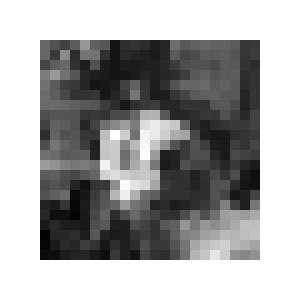
\includegraphics[width=\textwidth]{3_Reconocimiento/Figs/for_padding}
        \caption{Imagen original}
    \end{subfigure}
    \hfill
    \begin{subfigure}[t]{0.3\textwidth}
        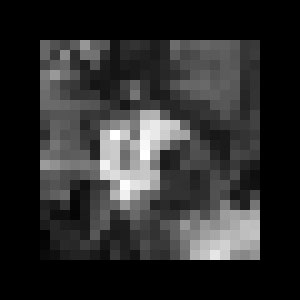
\includegraphics[width=\textwidth]{3_Reconocimiento/Figs/zero_padding}
        \caption{\emph{zero padding}}
    \end{subfigure}
    \hfill
    \begin{subfigure}[t]{0.3\textwidth}
        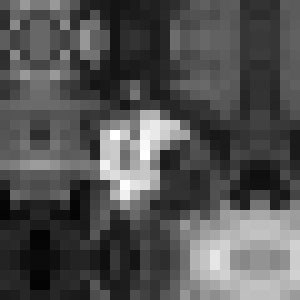
\includegraphics[width=\textwidth]{3_Reconocimiento/Figs/mirror_padding}
        \caption{\emph{mirror padding}}
    \end{subfigure}
    \caption*{\footnotesize Tomado de~\citep{Richard2011}.}
\end{figure}

El modo \emph{mirror} es utilizado para el filtro gaussiano y el \emph{zero} para adecuar la imagen antes del \hyperref[sec:segmentation]{paso 3} con el fin de completar el tamaño de $32 \times 32$ píxeles requerido para el \hyperref[sec:sift_descriptor]{paso 4}.

Como la imagen que contiene el dígito tendrá un tamaño diferente a $32 \times 32$, antes de efectuar el \emph{zero padding}, es necesario escalarla haciendo que el eje de mayor dimensión se ajuste a $32$ píxeles y el otro eje se ajuste proporcionalmente;
esta operación se lleva a cabo con la función \texttt{\small resize()} de \texttt{\small OpenCV}.
Luego sí se añaden los píxeles faltantes al eje de menor dimensión para completar los $32$ píxeles.
\vfill

\section*{Paso 3: Segmentación}
\label{sec:segmentation}
Existen diferentes técnicas de segmentación: basada en umbrales, en bordes, en regiones, por agrupación o por \emph{matching}.
Para los propósitos de este trabajo, es suficiente con una umbralización para discriminar los segmentos de la imagen, que corresponderían a los dígitos indicados en la pantalla del sonómetro.
Sin embargo, el umbral no puede ser el mismo para todas las imágenes, pues cada una puede estar influenciada por los efectos de iluminación, áreas o colores de los segmentos.
Una forma sistemática de determinar el umbral es empleando el algoritmo de \citet{Otsu1979}.
Este algoritmo busca maximizar la separación entre las clases de niveles de grises del histograma de la imagen usando los momentos de cero y primer orden.

La formulación de Otsu es un \emph{método no supervisado}\footnote{Los métodos no supervisados son aquellos que no requieren que las muestras de entrenamiento estén etiquetadas previamente según su clase, sino que a partir de los datos identifican patrones que permiten agruparlos.} basado en el análisis discriminante para evaluar la bondad del umbral y seleccionar automáticamente un límite óptimo.
En primer lugar, el método normaliza el histograma de niveles de grises y lo considera como una distribución de probabilidad.

Si hay $L$ niveles de grises, entonces el número de píxeles en la imagen es $N = n_1 + n_2 + \cdots + n_L$; $n_i$ es el número de píxeles que tienen un nivel $i$.
Luego, la distribución de probabilidad queda expresada como
%
\begin{equation}
    \label{eq:hist_p_distribution}
    p_i = \frac{n_i}{N}, \quad \text{en que } p_i \geq 0, \sum_{i = 1}^L p_i = 1.
\end{equation}

Ahora, se buscan dos clases $C_0$ y $C_1$, que corresponden a los píxeles que pertenecen al fondo y a los que pertenecen a los objetos, separados por el nivel de gris de valor $k$.
Las probabilidades de cada clase se definen de acuerdo con
%
\begin{subequations}
    \label{eq:otsu_class_probs}
    \begin{align}
        \omega_0 &= \mathrm{Pr}\left(C_0\right) = \sum_{i = 1}^k p_i = \omega(k); \label{eq:otsu_class_probs_1} \\
        \omega_1 &= \mathrm{Pr}\left(C_1\right) = 1 - \omega(k). \label{eq:otsu_class_probs2}
    \end{align}
\end{subequations}
%
Luego, los valores esperados condicionales de cada clase son:
%
\begin{subequations}
    \label{eq:otsu_expected_values}
    \begin{align}
        \mu_0 &= \sum_{i = 1}^k i\,\mathrm{Pr}\left(i|C_0\right) =
        \sum_{i = 1}^k i\,\frac{p_i}{\omega_0} = \frac{\mu(k)}{\omega(k)}; \label{eq:otsu_expected_values_1} \\
        \mu_1 &= \sum_{i = k + 1}^L i\,\mathrm{Pr}\left(i|C_i\right) =
        \sum_{i = k + 1}^L i\,\frac{p_i}{\omega_1} =
        \frac{\mu_T - \mu(k)}{1 - \omega(k)}. \label{eq:otsu_expected_values_2}
    \end{align}
\end{subequations}
%
En que $\omega(k)$ y $\mu(k)$ son los momentos acumulados de cero y primer orden del histograma hasta el $k$-ésimo nivel.
Estos momentos acumulados se definen como
%
\begin{subequations}
    \label{eq:otsu_cumulative_moments}
    \begin{align}
        \omega(k) &= \sum_{i = 1}^k p_i; \label{eq:otsu_cumulative_moments_1} \\
        \mu(k) &= \sum_{i = 1}^k i\,p_i.\label{eq:otsu_cumulative_moments_2}
    \end{align}
\end{subequations}

Similarmente, los momentos de primer y segundo orden de la imagen se definen como
%
\begin{subequations}
    \label{eq:otsu_total_moments}
    \begin{align}
        \mu_T &= \sum_{i = 1}^L i\,p_i; \label{eq:otsu_total_moments_1} \\
        \sigma_T^2 &= \sum_{i = 1}^L \left(i - \mu_T\right)^2\,p_i. \label{eq:otsu_total_moments_2}
    \end{align}
\end{subequations}
%
En que $\mu_T$ es la media total de los niveles de grises de la imagen original y $\sigma_T^2$ la varianza.

En principio, si las clases están separadas en sus niveles de grises entonces hay una umbralización adecuada.
Consecuentemente, un umbral que resulte en la mejor separación de clases según sus niveles de grises será un umbral óptimo.
Hay por lo menos tres medidas de separación entre clases que se pueden maximizar.
Sin embargo, por simplicidad (dado que depende de los momentos de orden cero y uno), conviene usar la medida definida en la siguiente ecuación como criterio para el análisis discriminante.
%
\begin{equation}
    \eta = \frac{\sigma_B^2}{\sigma_T^2}. \label{eq:otsu_discriminant_criterion}
\end{equation}
%
Donde el coeficiente $\sigma_B^2$ se define como
%
\begin{equation}
    \sigma_B^2 = \omega_0\,\omega_1\,\left(\mu_1 - \mu_0\right)^2. \label{eq:otsu_between_variance}
\end{equation}

Finalmente, condensando las ecuaciones (\ref{eq:otsu_expected_values}) a~\eqref{eq:otsu_between_variance}, el umbral óptimo $k^*$ que maximiza $\eta$ y, proporcionalmente, $\sigma_B^2$ se encuentra por medio de la siguiente expresión:
%
\begin{equation}
    \sigma_B^2(k^*) = \max_{1 \le k < L} \sigma_B^2(k). \label{eq:otsu_optimum_threshold}
\end{equation}
%
En la cual,
%
\begin{equation}
    \sigma_B^2(k) = \frac{\left[\mu_T\,\omega(k) - \mu(k)\right]^2}
    {\omega(k)\,\left[1 - \omega(k)\right]}. \label{eq:otsu_between_variance4optimize}
\end{equation}

Esta optimización se puede realizar de forma iterativa con unos valores iniciales de $\omega(0)$ y $\mu(0)$, luego iterando con todos los posibles valores de $k = 0, 1, \cdots, L$, y calculando $\sigma_B^2(k)$.
El umbral óptimo $k^*$ será el máximo valor obtenido de $\sigma_B^2(k)$.


\section*{Paso 4: Descriptor local SIFT}
\label{sec:sift_descriptor}
En esta aplicación particular (cuyo funcionamiento se pretende en tiempo real), el objeto de reconocimiento es simple, por lo que no hace falta el sofisticado algoritmo de detección, localización y orientación de puntos característicos de la presentación original del descriptor SIFT propuesto por \citet{Lowe2004}.
No obstante, la implementación del algoritmo aquí presentada sí tiene en cuenta su propuesta de descriptor local basada en la magnitud y dirección de los gradientes de cada píxel perteneciente a la región alrededor de cada punto característico.

En primer lugar, se calcula la magnitud y dirección del gradiente de cada píxel.
Esto finalmente es una valoración del cambio direccional en la intensidad de la imagen.
La dirección final del gradiente en un píxel es aquella en la que ocurre el máximo cambio de intensidad, y la magnitud sería el máximo cambio de intensidad.
Para lo cual se emplean las siguientes ecuaciones:
%
\begin{subequations}
    \label{eq:sift_gradient}
    \begin{align}
        \delta_x &= I(x + 1, y) - I(x - 1, y); \label{eq:sift_gradient_1} \\
        \delta_y &= I(x, y + 1) - I(x, y - 1); \label{eq:sift_gradient_2} \\
        \theta(x,y) &= \tan^{-1}\left(\frac{\delta_y}{\delta_x}\right); \label{eq:sift_gradient_3} \\
        |\nabla f(x, y)| &= \sqrt{\delta_x^2 + \delta_y^2}. \label{eq:sift_gradient_4}
    \end{align}
\end{subequations}

Las diferencias de intensidad en $x$ y en $y$ se determinan con las ecuaciones~\eqref{eq:sift_gradient_1} y~\eqref{eq:sift_gradient_2}, luego, la dirección con~\eqref{eq:sift_gradient_3} y la magnitud con~\eqref{eq:sift_gradient_4}.

Después de obtener todas las magnitudes y direcciones de los gradientes, se conforma un histograma de orientaciones en $8$ intervalos por cada ventana de $n \times n = 4 \times 4$ píxeles;
es decir, según la dirección de cada vector, su magnitud se suma en el respectivo intervalo del histograma de la ventana al que pertenece.
Finalmente, queda un vector de características de $128$ valores que es la concatenación de todos los histogramas, cada uno de $8$ valores.
Pero la contribución de esta magnitud a su intervalo de orientación correspondiente es ponderada por la función gaussiana de la ecuación~\eqref{eq:sift_gaussian_weighting} con $\sigma$ igual a la mitad del ancho de la ventana del descriptor, con el propósito de dar menor peso a los gradientes que están más lejos del centro del descriptor.
%
\begin{equation}
    \label{eq:sift_gaussian_weighting}
    G(x,y) = \frac{1}{2\,\pi\,\sigma^2}\,\exp{\left(-\frac{x^2 + y^2}{2\,\sigma^2}\right)  }.
\end{equation}

El objetivo del histograma es permitir que haya cambios locales más grandes en las direcciones de los gradientes, pero que contribuyan al mismo intervalo en el histograma.
Ahora bien, pueden ocurrir cambios abruptos en el histograma cuando en realidad hay cambios suaves en las direcciones de las muestras de gradientes, esto debido a los efectos de los límites en los intervalos.
Para mitigar este efecto, se aplica una interpolación trilineal\footnote{La interpolación trilineal es la extensión de la interpolación lineal a un espacio tridimensional ($D = 3$) usando polinomios de primer orden. En la práctica resulta ser la interpolación lineal de dos interpolaciones bilineales. Con esta operación se encuentra un valor intermedio teniendo en cuenta los $2^D$ valores adyacentes.} para distribuir la magnitud de cada muestra de gradiente en intervalos de histograma adyacentes, en función de la ``distancia'' de la dirección de la muestra desde el valor central del intervalo.
Esto queda reflejado en las siguientes funciones de ponderación:
%
\begin{subequations}
    \begin{align}
        w_k(x, y) &= \left\{\begin{matrix}
                                \nabla\theta(x, y),     & \text{si } k = i\theta(x, y)       \\
                                1 - \nabla\theta(x, y), & \text{si } k = i\theta \bmod 8 + 1 \\
                                0,                      & \text{en caso contrario}
        \end{matrix} \right. \label{eq:sift_trilineal_weighting_1} \\
        w_i(x, y) &= \left\{\begin{matrix}
                                \nabla x(x, y),     & \text{si } i = ix(x, y)     \\
                                1 - \nabla x(x, y), & \text{si } i = ix(x, y) + 1 \\
                                0,                  & \text{en caso contrario}
        \end{matrix} \right. \label{eq:sift_trilineal_weighting_2} \\
        w_j(x, y) &= \left\{\begin{matrix}
                                \nabla y(x, y),     & \text{si } j = iy(x, y)     \\
                                1 - \nabla y(x, y), & \text{si } j = iy(x, y) + 1 \\
                                0,                  & \text{en caso contrario}
        \end{matrix} \right. \label{eq:sift_trilineal_weighting_3}
    \end{align}
\end{subequations}
%
Con las siguientes definiciones:
\begin{subequations}
    \begin{align}
        \nabla\theta(x, y) &= i\theta(x, y) - \frac{\theta(x, y)}{\delta\theta}, \quad \text{en que }
        i\theta(x, y) = \left\lceil \frac{\theta(x, y)}{\delta\theta} \right\rceil \text{y } \delta\theta = 360 / n; \\
        \nabla x(x, y) &= ix(x, y) - \frac{x}{\delta x}, \quad \text{en que } ix(x, y) = \left\lceil \frac{x}{\delta x} \right\rceil; \\
        \nabla y(x, y) &= iy(x, y) - \frac{y}{\delta x}, \quad \text{en que } iy(x, y) = \left\lceil \frac{y}{\delta x} \right\rceil.
    \end{align}
\end{subequations}

En seguida, se conforma el histograma como se presenta a continuación:
%
\begin{align}
    H &= \left(H_{11}, H_{12}, \cdots, H_{nn} \right); \nonumber \\
    H_j &= \left(h_1, h_2, \cdots, h_n\right); \nonumber \\
    h_{k}(x, y) &=
    \sum_{(x, y)} w_k(x, y)\,w_i(x, y)\,w_j(x, y)\,|\nabla f(x, y)|\,G(x, y).
\end{align}

Finalmente el arreglo resultante se normaliza para hacerlo invariante a los efectos de contrastes o cambios en la iluminación, y para reducir los efectos de cambios no lineales en iluminación debidos a la saturación de la cámara, se limitan los valores con un umbral experimental de $\num{0.2}$, de manera que los valores inferiores a $\num{0.2}$ son remplazados con $\num{0.2}$, y se normaliza nuevamente.
La normalización se efectúa empleando la norma $L_2$, como se muestra a continuación:
%
\begin{subequations}
    \begin{align*}
        H &= \left(H_{11}, H_{12}, \cdots, H_{nn}\right) \Rightarrow v = \left(v_1, v_2, \cdots, v_m\right). \\
        \|v\|_2 &= \sqrt{\sum_{i = 1}^m v_i^2}. \\
        v' &= \left(\frac{v_1}{\|v\|_2}, \frac{v_2}{\|v\|_2}, \cdots, \frac{v_m}{\|v\|_2}\right); \\
        v'' &= \left(\max\left(v_1, 0.2\right), \max\left(v_2, 0.2\right), \cdots, \max\left(v_m, 0.2\right)\right); \\
        v''' &= \frac{v''}{\|v''\|_2}.
    \end{align*}
\end{subequations}

\section*{Paso 5: Reducción de dimensionalidad por análisis de componentes principales (KPCA)}
\label{sec:kpca_reduction}
Una vez se obtienen los vectores de características de las muestras, conviene un proceso adicional para simplificar el análisis posterior de los datos, mejorar el desempeño en la clasificación, eliminar información redundante o incluso poder obtener representaciones gráficas de los vectores.
Generalmente, los vectores de características resultan ser de grandes dimensiones, lo que provoca ciertas desventajas como que al aumentar las dimensiones de los vectores el volumen del espacio aumenta exponencialmente y los datos tienden a volverse dispersos, y esto afecta negativamente la clasificación, pues los datos se organizan en áreas correspondientes a grupos con características similares, y finalmente las estrategias comunes de clasificación no son eficaces.
Ese efecto llamado "la maldición de la dimensión" puede ser abordado con diferentes métodos, entre estos la reducción de dimensionalidad tomando las componentes principales del grupo de datos usando el truco del \emph{kernel} (KPCA) originalmente propuesto por \citet{Scholkopf1997}.

En principio se toma el método de análisis de componentes principales (PCA), en el que básicamente se hace una transformación euclidia al rotar y trasladar los ejes para alcanzar la mayor variabilidad descendentemente en todas las dimensiones.
En la práctica, se trazan planos de modo que las distancias de los puntos a estos sean las mínimas posibles.
Las componentes principales corresponden a las primeras dimensiones del hiperplano resultante, en las que se encuentra la mayor variabilidad.
Para lograr esto se diagonaliza la matriz de covarianza de los datos $\vect{x}_k \in \vect{R}^N$, con $k = 1, \cdots, \ell$ definida en~\eqref{eq:kpca_covariance}.
Los datos están centrados en el origen, de modo que $\sum_{k = 1}^\ell \vect{x}_k = 0$.
%
\begin{equation}
    \label{eq:kpca_covariance}
    \vect{C} = \frac{1}{\ell} \sum_{j = 1}^\ell \vect{x}_j\,\vect{x}_j^\top.
\end{equation}

La diagonalización, en otras palabras, es una descomposición en valores y vectores propios de la matriz $\vect{C}$, y las proyecciones ortogonales de los puntos en los eigenvectores son las componentes principales.

Ahora, suele ocurrir que la separación entre los datos no es del todo lineal y entonces es necesario hacer una transformación no lineal de los datos a un nuevo espacio de características $\mathcal{F}$, como se describe a continuación:
%
\begin{equation}
    \label{eq:kpca_non-linear_mapping}
    \Phi: \vect{R}^N \to \mathcal{F}, \quad \vect{x} \mapsto \vect{X}.
\end{equation}

En ese nuevo espacio $\mathcal{F}$ también es posible hacer el análisis PCA. La transformación se realiza usando \emph{kernels}, que son funciones continuas conocidas del método de las máquinas de vectores de soporte (SVM), que además mejoran el costo computacional, porque el cálculo depende del producto interno de los vectores en el nuevo espacio, i.e $\vect{k}(\vect{x}, \vect{x}') = \Phi\left(\vect{x}\right)^\top\cdot\Phi\left(\vect{x'}\right)$.

Luego, si en el espacio original el análisis PCA se hacía con la descomposición de $\lambda\,\vect{x}_k\,\vect{V} = \vect{x}_k\,\vect{C}\,\vect{V}$, en el nuevo espacio de características, equivalentemente se hace la descomposición del sistema
%
\begin{equation}
    \label{eq:kpca_eigendecomposition}
    \lambda\left(\Phi\left(\vect{x}_k\right)\cdot\vect{V}\right) =
    \left(\Phi\left(\vect{x}_k\right)\cdot\bar{\vect{C}}\,\vect{V}\right), \quad \forall k = 1, \cdots, \ell.
\end{equation}
%
Con $\bar{\vect{C}} = \frac{1}{\ell}\sum_{j = 1}^\ell \Phi\left(\vect{x}_j\right)\,\Phi\left(\vect{x}_j\right)^\top$.

Luego, el vector propio puede ser expresado como una combinación lineal de los datos transformados:
%
\begin{subequations}
    \begin{align}
        \vect{V} &= \frac{1}{\ell\,\lambda} \sum_{i = 1}^\ell \left(
        \Phi\left(\vect{x}_i\right)\cdot\vect{V}\right)\,\Phi\left(\vect{x}_i\right); \\
        \vect{V} &= \sum_{i = 1}^\ell \alpha_i\,\Phi\left(\vect{x}_i\right). \label{eq:kpca_alpha}
    \end{align}
\end{subequations}

Ahora, para generar el producto interno de los vectores, se multiplica a ambos lados de~\eqref{eq:kpca_alpha} por $\Phi\left(\vect{x}_j\right)$, y se obtiene
%
\begin{equation}
    \label{eq:kpca_internal_product}
    \vect{V}\cdot\Phi\left(\vect{x}_j\right) = \lambda\,\ell\,\alpha_j
    \quad = \quad \sum_{i = 1}^\ell \alpha_i\,\left(\Phi\left(\vect{x}_i\right)\cdot\Phi\left(\vect{x}_j\right)\right)
    = \sum_{i = 1}^\ell \alpha_i\,\vect{K}_j.
\end{equation}
%
Recordando que $\vect{K}_j \defeq  \Phi\left(\vect{x}_i\cdot\Phi\left(\vect{x}_j\right)\right)$.

Finalmente, expresando~\eqref{eq:kpca_internal_product} de forma vectorial y matricial se llega a que el problema de eigenvalores a resolver es:
%
\begin{equation}
    \ell\,\lambda\,\boldsymbol{\alpha} = \vect{K}\,\boldsymbol{\alpha}.
\end{equation}

De este modo, los valores propios de $\vect{K}$ son proporcionales a los valores propios de $\bar{\vect{C}}$ y la extracción de características se haría tomando los eigenvalores más grandes.

Como funciones de \emph{kernel} pueden usarse diferentes funciones (e.g.\ polinomial, sigmoide, etc).
En este caso, se utilizó uno de base radial como el \emph{kernel} gaussiano que se presenta en la siguiente ecuación:
%
\begin{equation}
    \label{eq:kpca_gaussian}
    \vect{k}\left(\vect{x}, \vect{y}\right) = e^{\left(-\frac{\|\vect{x} - \vect{y}\|^2}{2\,\sigma^2}\right)}.
\end{equation}

\section*{Paso 6: Clasificador bayesiano normal}
\label{sec:nb_classifier}
En la última etapa de un sistema de visión de máquina se encuentra el reconocimiento e interpretación, en la cual se utilizan diversas técnicas.
Una de las más clásicas es el clasificador paramétrico supervisado basado en la teoría de decisión de Bayes formulada de forma general a continuación.
%
\begin{equation}
    \label{eq:bayes_general_formula}
    P(A|B) = \frac{P(A)\,P(B|A)}{P(B)}.
\end{equation}
%
En la que se toma $A$ como hipótesis y $B$ como la evidencia.

Generalmente, se hacen simplificaciones en el modelo asumiendo que hay independencia entre las características de entrada, de manera tal que se asume que la presencia o ausencia de una característica no afecta a las otras, entonces cada característica contribuye independientemente a la probabilidad del evento $A$.
A este caso se le llama \emph{clasificador ingenuo}.

Ahora, en términos de clases $\left(y_i\right)$ y características $\left(\vect{X}\right)$ , la ecuación~\eqref{eq:bayes_general_formula} puede ser expresada como
%
\begin{subequations}
    \begin{align}
        P\left(y_i|\vect{X}\right) &= \frac{P\left(y_i\right)\,P(\vect{X}|y_i)}{P(\vect{X})}; \\
        P\left(y_i | \vect{x}_1, \dots, \vect{x}_n\right) &=
        \frac{P\left(y_i\right)\,P\left(\vect{x}_1, \dots, \vect{x}_n | y_i\right)}
        {P\left(\vect{x}_1, \dots, \vect{x}_n\right)}. \label{eq:bayes_features_formula}
    \end{align}
\end{subequations}

Al asumir la independencia entre las características de entrada, es posible reescribir~\eqref{eq:bayes_features_formula} usando la regla de la cadena, y queda que
%
\begin{equation}
    \label{eq:bayes_features_prod}
    P\left(y_i | \vect{x}_1, \dots, \vect{x}_n\right) =
    \frac{P\left(y_i\right) \prod_{j = 1}^n P\left(\vect{x}_j | y_i\right)}
    {P\left(\vect{x}_1, \dots, \vect{x}_n\right)}.
\end{equation}

En la práctica, el denominador de~\eqref{eq:bayes_features_prod} permanece constante, y como además no depende de la clase, puede omitirse y queda que la probabilidad de una clase $y_i$ dadas las características $\vect{X}$ es proporcional a la productoria, es decir,
%
\begin{equation}
    \label{eq:bayes_prop_prod}
    P\left(y_i | \vect{x}_1, \dots, \vect{x}_n\right) \propto
    P\left(y_i\right) \prod_{j = 1}^n P\left(\vect{x}_j | y_i\right).
\end{equation}

Finalmente, la clase por la que se decide el clasificador es aquella que tiene mayor probabilidad, como se define en la siguiente expresión:
%
\begin{equation}
    \label{eq:bayes_clasifier}
    \hat{y} = \arg\max_{y_i} \, P\left(y_i\right) \prod_{j = 1}^n P\left(\vect{x}_j | y_i\right).
\end{equation}

Ahora, tanto los parámetros del modelo, como las clases a priori y las características de las distribuciones de probabilidad, se determinan sobre el conjunto de datos de entrenamiento.
Los parámetros del modelo se determinan haciendo estimaciones de máxima verosimilitud, maximizando la función de distribución de probabilidad, i.e.\ derivando respecto a cada parámetro e igualando a $0$.

Cuando los datos pueden tomar valores de una función continua, generalmente se asume que siguen una distribución normal, la cual se presenta su versión multivariada en la siguiente expresión:
%
\begin{align}
    p(\vect{x}_k) &\sim N(\boldsymbol{\mu}, \boldsymbol{\Sigma}); \nonumber \\
    &\sim \frac{1}{(2\,\pi)^{d/2}\left|\boldsymbol{\Sigma}\right|^{1/2}}\,
    \exp\left(-\frac{1}{2}\left(\vect{x}_k - \boldsymbol{\mu}\right)^\top\,
    \boldsymbol{\Sigma}^{-1}\,\left(\vect{x}_k - \boldsymbol{\mu}\right)\right). \label{eq:gaussian_bayes}
\end{align}

En la estimación de máxima verosimilitud (MLE), con el fin de maximizar la función y encontrar los parámetros de la distribución, conviene operar\eqref{eq:gaussian_bayes}) expresada en funciones monótonamente crecientes como el logaritmo natural y la suma, lo que se denomina \emph{log-verosimilitud}, como se muestra a continuación.
%
\begin{equation}
    \label{eq:gaussian_log-likehood}
    \ell(\boldsymbol{\theta}) = \sum_{k = 1}^n - \frac{1}{2}\left(\vect{x}_k -
    \boldsymbol{\mu}\right)^\top\,\boldsymbol{\Sigma}^{-1}\,\left(\vect{x}_k - \boldsymbol{\mu}\right)
    - \frac{d}{2}\,\ln{2\,\pi} - \frac{1}{2}\,\ln{\left|\boldsymbol{\Sigma}\right|}.
\end{equation}

Los parámetros a encontrar son $\theta_1 = \boldsymbol{\mu}$ y $\theta_2 = \boldsymbol{\Sigma}$, que al hacer la maximización de \eqref{eq:gaussian_log-likehood} quedan definidos como
%
\begin{subequations}
    \begin{align}
        \hat{\theta}_1 &= \hat{\boldsymbol{\mu}} = \frac{1}{n}\,\sum_{k = 1}^n \vect{x}_k; \label{eq:gaussian_mu}\\
        \hat{\theta}_2 &= \hat{\boldsymbol{\Sigma}} =
        \frac{1}{n} \,\sum_{k = 1}^n \left(\vect{x}_k - \hat{\boldsymbol{\mu}}\right)
        \left(\vect{x}_k - \hat{\boldsymbol{\mu}}\right)^\top. \label{eq:gaussian_Sigma}
    \end{align}
\end{subequations}

Para conformar el clasificador normal bayesiano, en primer lugar se asume que cada clase tiene una distribución normal de la misma forma que la ecuación\eqref{eq:gaussian_bayes}), y sus parámetros $\boldsymbol{\mu}$ y $\boldsymbol{\Sigma}$ dependen de los datos que, en la etapa de entrenamiento, se ha determinado que describen la distribución normal de cada clase.
Y entonces la ecuación~\eqref{eq:gaussian_bayes} pasa a ser la probabilidad de $\vect{x}_j$ dada una clase $y_i$, cuyos parámetros de distribución de probabilidad están dados por:
%
\begin{subequations}
    \begin{align}
        \boldsymbol{\mu}_i &= \frac{1}{n_i}\,\sum_{j = 1}^{n} z_{ij}\,\vect{x}_j, \quad \text{en que }
        z_{ij} = \left\{\begin{matrix}
                            1, & \text{si } \vect{x}_j \in y_i \\
                            0, & \text{si no}
        \end{matrix}\right.;\label{eq:gaussian_mean_class} \\
        \boldsymbol{\Sigma}_i &= \frac{1}{n_i}\,\sum_{j = 1}^{n} z_{ij}\,
        \left(\vect{x}_j - \boldsymbol{\mu}_i\right)\,
        \left(\vect{x}_j - \boldsymbol{\mu}_i\right)^\top, \quad \text{en que }
        z_{ij} = \left\{\begin{matrix}
                            1, & \text{si } \vect{x}_j \in y_i \\
                            0, & \text{si no}
        \end{matrix}\right..\label{eq:gaussian_Sigma_class}
    \end{align}
\end{subequations}

Con estas probabilidades condicionales se combina~\eqref{eq:gaussian_bayes} con~\eqref{eq:bayes_clasifier}; primero definiendo las funciones discriminantes con \emph{log-verosimilitud} como
%
\begin{align}
    g_i(\vect{x}) &= \ln{p\left(\vect{x}|y_i\right)} + \ln{P\left(y_i\right)}; \nonumber \\
    &= - \frac{1}{2}\left(\vect{x} - \boldsymbol{\mu}_i\right)^\top\,\boldsymbol{\Sigma}_i^{-1}\,
    \left(\vect{x} - \boldsymbol{\mu}_i\right) - \frac{d}{2}\,\ln{2\,\pi}
    - \frac{1}{2}\,\ln{\left|\boldsymbol{\Sigma}_i\right|} + \ln{P\left(y_i\right)}. \label{eq:gaussian_discriminant_function}
\end{align}

Finalmente, la función~\eqref{eq:gaussian_discriminant_function} se utiliza para decidir la clase a la que pertenecen las características $\vect{x} = x_1, \dots, x_d$ de una muestra dada.
La clase de salida nuevamente es la que tenga la mayor probabilidad, es decir:
%
\begin{equation}
    \hat{y} = \arg\max_{y_i} g_i(\vect{x}).
\end{equation}
\vfill

\section*{Resultados}

A continuación se presentarán algunos detalles en la implementación de los procesamientos presentados en las secciones anteriores y ejemplos de los resultados.
Las imágenes del conjunto de entrenamiento y de prueba fueron obtenidas fotografiando la pantalla de un sonómetro marca 01dB, modelo CUBE. Un ejemplo se muestra en la siguiente figura.
%
\begin{figure}[h]
    \caption{Ejemplo de una fotografía de la pantalla de un sonómetro 01dB CUBE.}
    \label{fig:slm_screen}
    \centering
    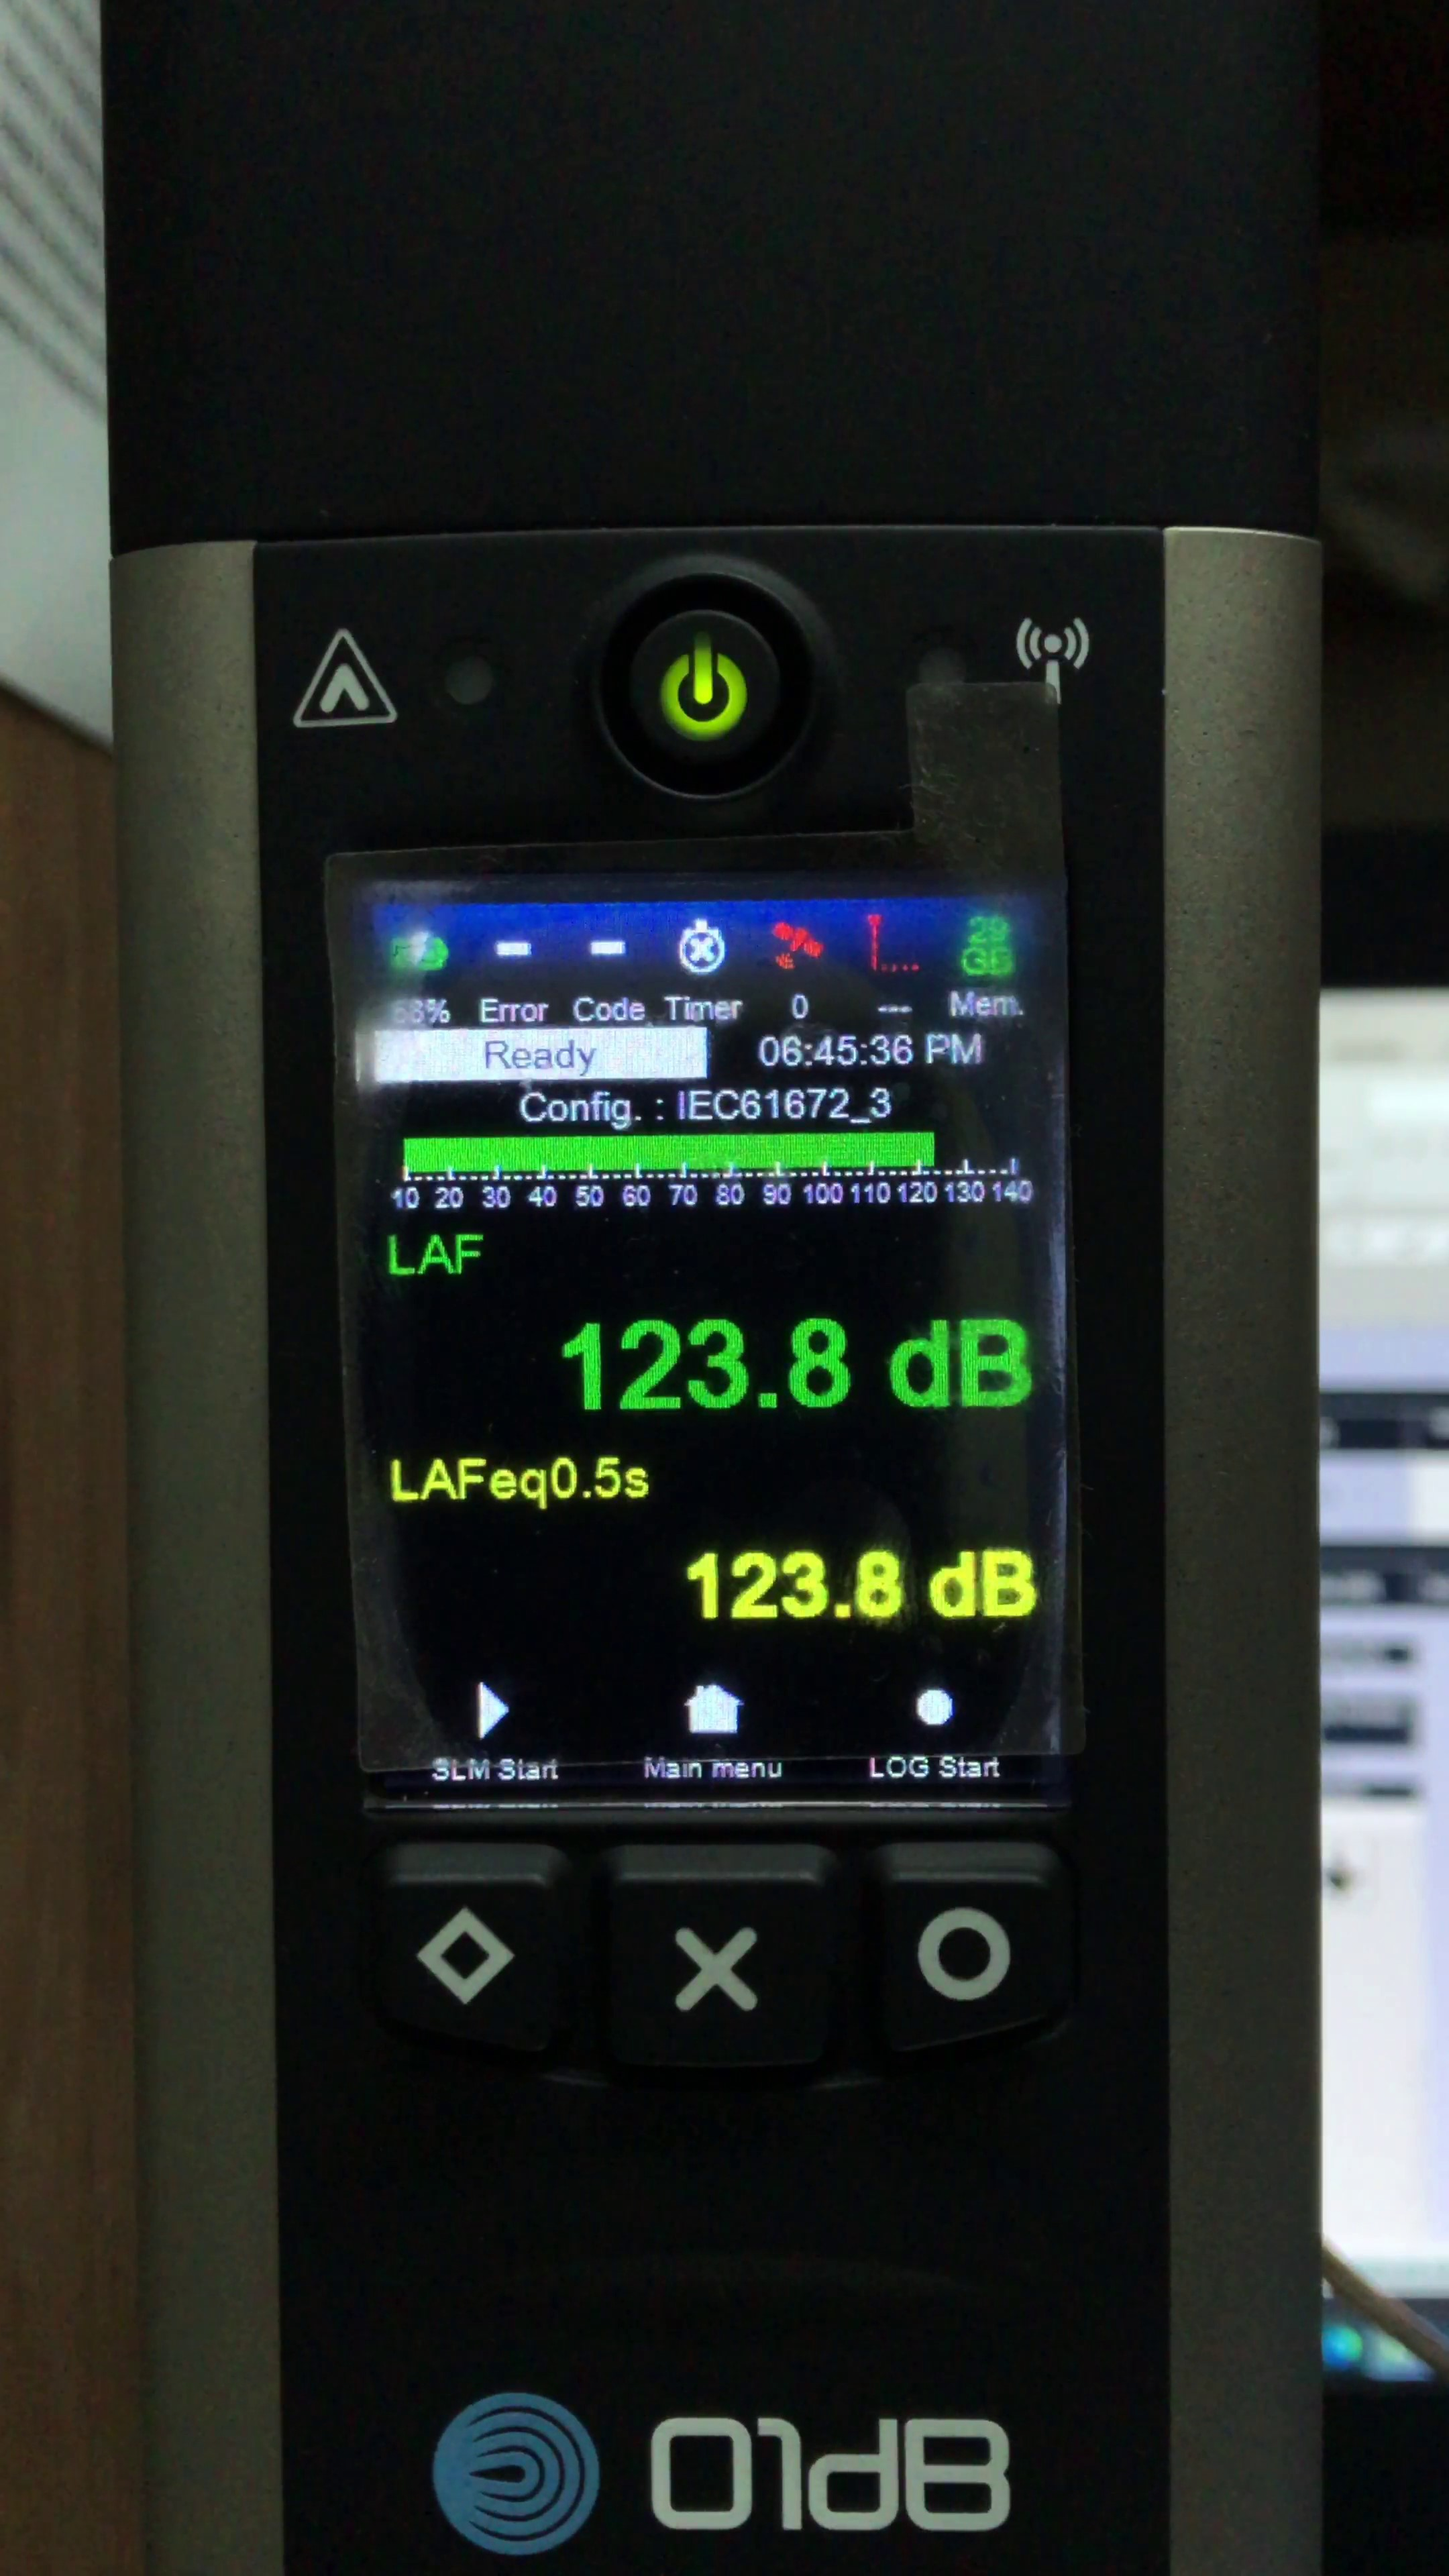
\includegraphics[height=7.2cm]{3_reconocimiento/Figs/slm_screen}
\end{figure}

Para el filtro gaussiano se empleó $\sigma_x = \sigma_y = \num{1.5}$.
Luego, con el fin de simplificar el cálculo del descriptor SIFT, se escala la imagen de un dígito y se rellenan los píxeles faltantes para conformar una imagen de $32 \times 32$.
Después, se eligen cuatro puntos clave que corresponden a los centros de cada cuadrante como se presenta en la siguiente figura.
%
\begin{figure}[h]
    \caption{Puntos clave para el cálculo del descriptor SIFT de una imagen de un dígito.}
    \label{fig:keypoints_SIFT}
    \centering
    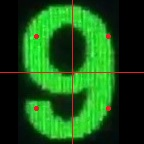
\includegraphics[height=5cm]{3_Reconocimiento/Figs/keypoints_SIFT}
\end{figure}

En esos puntos se calcula el descriptor SIFT, no sin previamente haber umbralizado la imagen redimensionada con el método de Otsu.
De forma tal que queda un vector de características con $512$ valores para cada muestra.

Una breve implementación de este procesamiento se presenta en el código~\ref{code:test_samples_code}, que posteriormente será usado en la aplicación desarrollada para automatizar la calibración de sonómetros.

En la siguiente figura se muestran los resultados de los pasos 1 al 3 del algoritmo~\ref{alg:image_recongnition} para una muestra de entrenamiento del número $5$.
%
\tikzmath{\x1 = 6.3;}
\begin{figure}[hb!]
    \caption{Resultados de procesamiento de una muestra de entrenamiento del número $5$.}
    \label{fig:train_sample5_processing}
    \centering
    \begin{subfigure}[t]{0.48\textwidth}
        \centering
        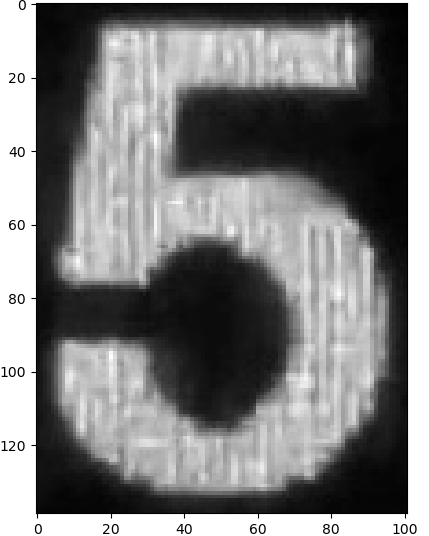
\includegraphics[height=\x1cm]{3_Reconocimiento/Figs/train_sample5_original}
        \caption{Imagen original en escala de grises.}
    \end{subfigure}
    \hfill
    \begin{subfigure}[t]{0.48\textwidth}
        \centering
        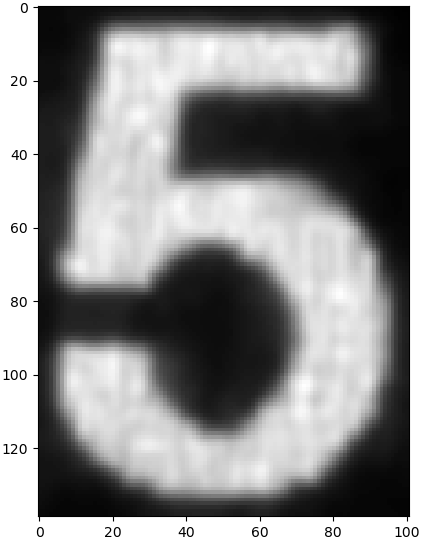
\includegraphics[height=\x1cm]{3_Reconocimiento/Figs/train_sample5_filtered}
        \caption{Imagen filtrada con filtro gausiano \hyperref[sec:gaussian_filter]{(paso 1)}.}
    \end{subfigure}
    \\[+1em]
    \begin{subfigure}[t]{0.48\textwidth}
        \centering
        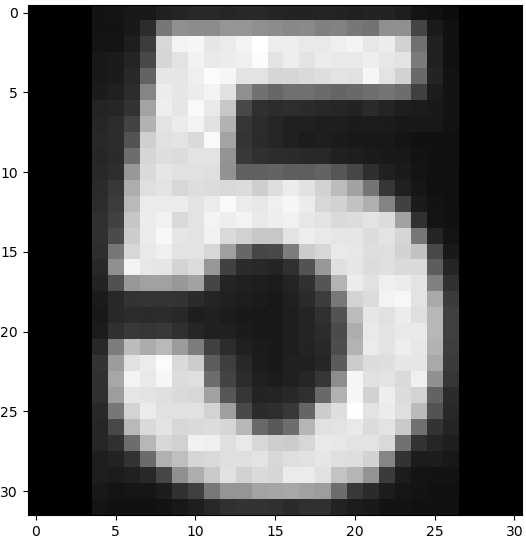
\includegraphics[height=\x1cm]{3_Reconocimiento/Figs/train_sample5_padded}
        \caption{Imagen escalada y con \emph{padding} \hyperref[sec:padding]{(paso 2)}.}
    \end{subfigure}
    \hfill
    \begin{subfigure}[t]{0.48\textwidth}
        \centering
        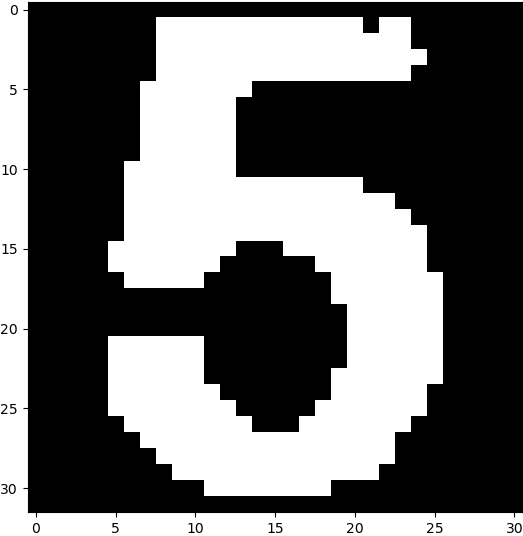
\includegraphics[height=\x1cm]{3_Reconocimiento/Figs/train_sample5_otsu}
        \caption{Imagen binarizada con el método de Otsu \hyperref[sec:segmentation]{(paso 3)}}
    \end{subfigure}
\end{figure}

Para el \hyperref[sec:sift_descriptor]{paso 4}, con las últimas líneas del código~\ref{code:test_samples_code} también se grafican los vectores de características.
En la figura~\ref{fig:train_samples_features} se muestran los resultados de una muestra de cada clase $2$, $5$ y $7$.
%
\begin{figure}[h]
    \caption{Vectores de características de una muestra de cada clase $2$, $5$ y $7$.}
    \label{fig:train_samples_features}
    \centering
    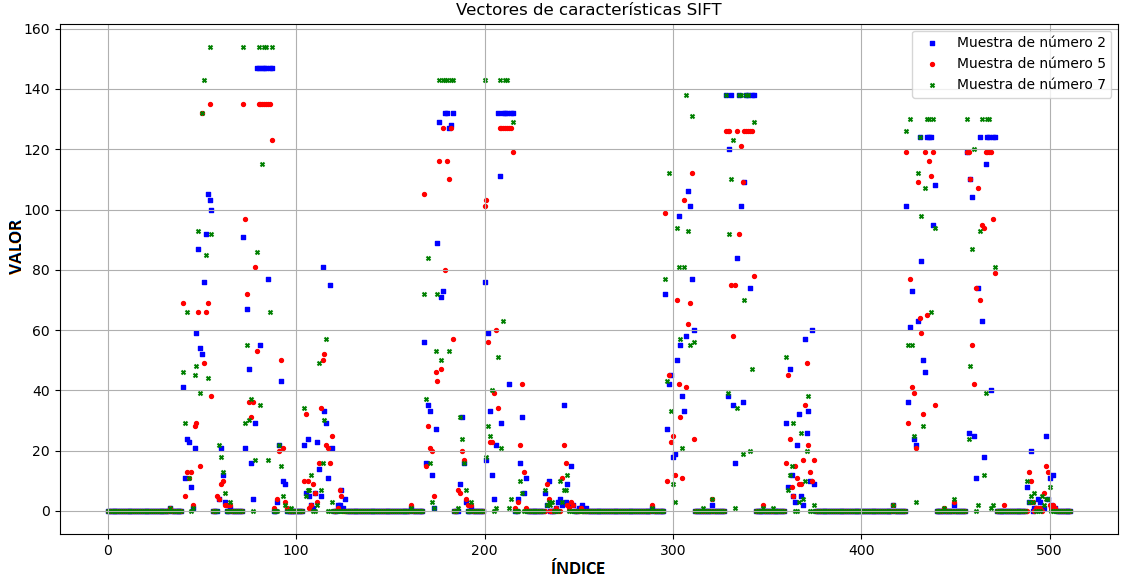
\includegraphics[width=0.8\textwidth]{3_Reconocimiento/Figs/train_samples_features}
\end{figure}

Ahora, el código~\ref{code:test_samples_code} se puede ejecutar iterativamente para leer todas las imágenes de un conjunto de entrenamiento con aproximadamente entre $40$ y $100$ muestras por cada clase.
Luego, para los pasos \hyperref[sec:kpca_reduction]{5} y \hyperref[sec:nb_classifier]{6}, complementando con el código~\ref{code:features_extracting}, se efectúa la extracción de características y se entrena el clasificador bayesiano normal.
La reducción de dimensionalidad se hizo hasta un valor de $d = 16$, empíricamente seleccionado según los resultados de clasificación obtenidos.

Finalmente, para una muestra dada de prueba, se efectúa el mismo procesamiento de la imagen con el código~\ref{code:test_samples_code}, y la extracción y clasificación se efectúa con el código~\ref{code:sample_classifying}.

Durante los primeros ensayos del algoritmo se pudo notar que si las condiciones de captura de la imagen no son controladas, factores como el desenfoque de la cámara, la alta exposición controlada por el diafragma de la cámara, reflejos, destellos de luz o bajo contraste, pueden afectar significativamente la clasificación.
Por ejemplo, en la figura~\ref{fig:good_bad_conditions} se presenta una comparación entre tres números fotografiados en condiciones controladas y no controladas, y el respectivo resultado de procesamiento.

\tikzmath{\x1 = 5.3;}
\begin{figure}[hp!]
    \caption{Comparación del procesamiento de imágenes tomadas en condiciones controladas y no controladas.}
    \label{fig:good_bad_conditions}
    \centering
    \begin{subfigure}[t]{0.3\textwidth}
        \centering
        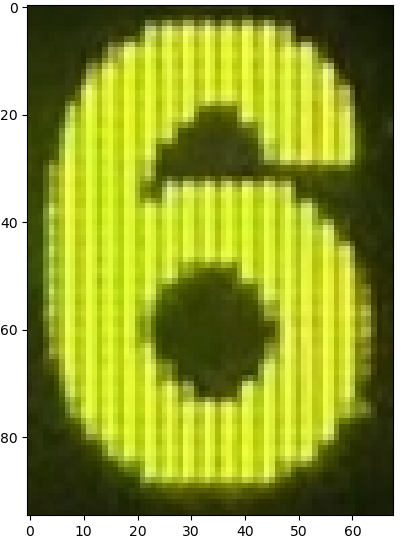
\includegraphics[height=\x1cm]{3_Reconocimiento/Figs/test_sample6_good_original}
        \caption{Imagen original en condiciones controladas.}
        \label{fig:good_conditions_original}
    \end{subfigure}
    \hfill
    \begin{subfigure}[t]{0.3\textwidth}
        \centering
        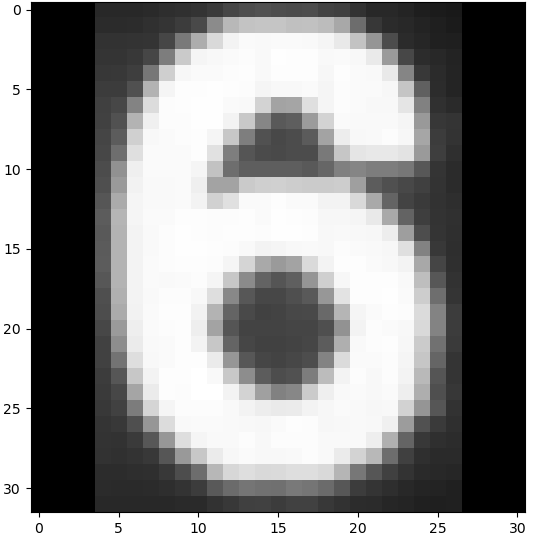
\includegraphics[height=\x1cm]{3_Reconocimiento/Figs/test_sample6_good_padded}
        \caption{Imagen hasta el paso 2 en condiciones controladas.}
        \label{fig:good_conditions_padded}
    \end{subfigure}
    \hfill
    \begin{subfigure}[t]{0.3\textwidth}
        \centering
        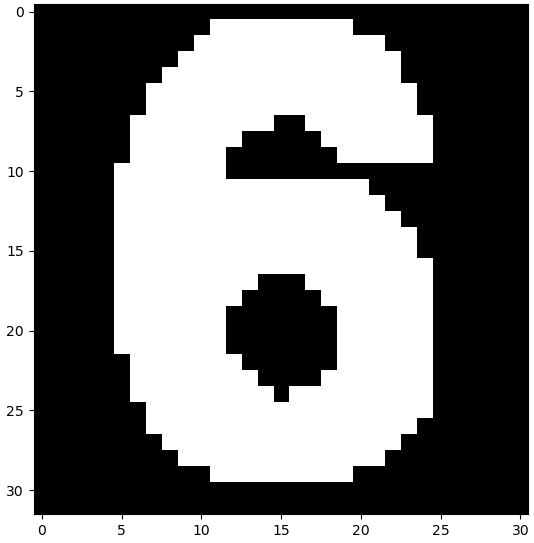
\includegraphics[height=\x1cm]{3_Reconocimiento/Figs/test_sample6_good_otsu}
        \caption{Imagen hasta el paso 3 en condiciones controladas.}
    \end{subfigure}
    \\[+1em]
    \begin{subfigure}[t]{0.3\textwidth}
        \centering
        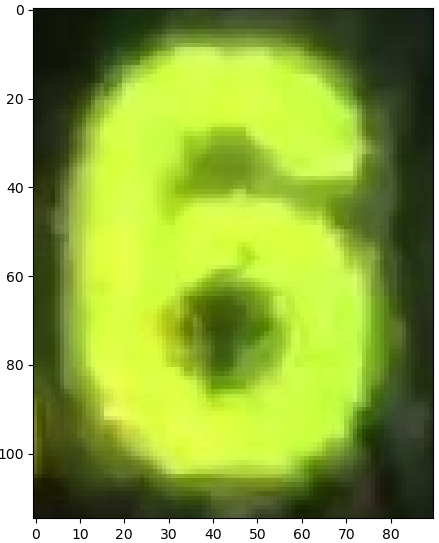
\includegraphics[height=\x1cm]{3_Reconocimiento/Figs/test_sample6_bad_original1}
        \caption{Imagen original en condiciones no controladas.}
    \end{subfigure}
    \hfill
    \begin{subfigure}[t]{0.3\textwidth}
        \centering
        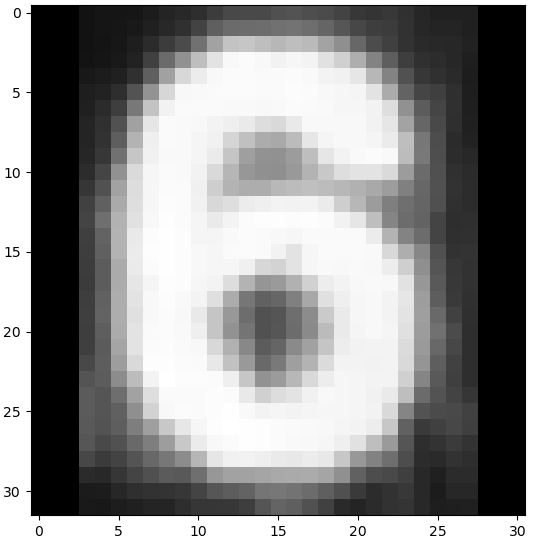
\includegraphics[height=\x1cm]{3_Reconocimiento/Figs/test_sample6_bad_padded1}
        \caption{Imagen hasta el paso 2 en condiciones no controladas.}
    \end{subfigure}
    \hfill
    \begin{subfigure}[t]{0.3\textwidth}
        \centering
        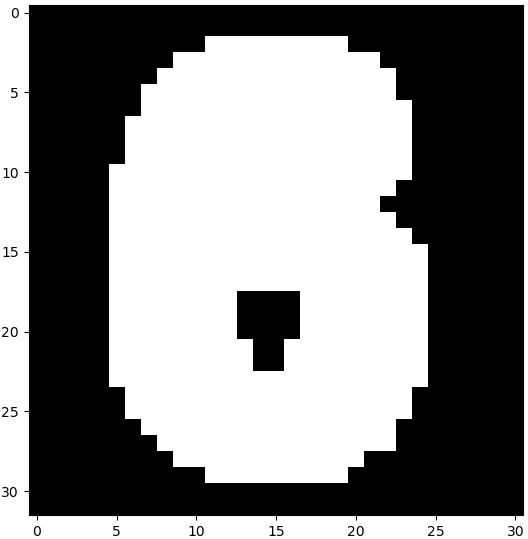
\includegraphics[height=\x1cm]{3_Reconocimiento/Figs/test_sample6_bad_otsu1}
        \caption{Imagen hasta el paso 3 en condiciones no controladas.}
    \end{subfigure}
    \\[+1em]
    \begin{subfigure}[t]{0.3\textwidth}
        \centering
        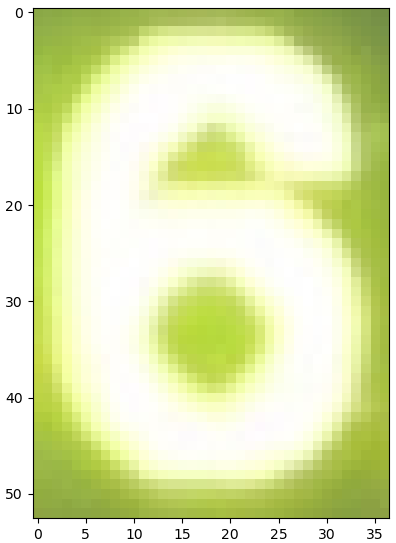
\includegraphics[height=\x1cm]{3_Reconocimiento/Figs/test_sample6_bad_original2}
        \caption{Imagen original en condiciones no controladas.}
    \end{subfigure}
    \hfill
    \begin{subfigure}[t]{0.3\textwidth}
        \centering
        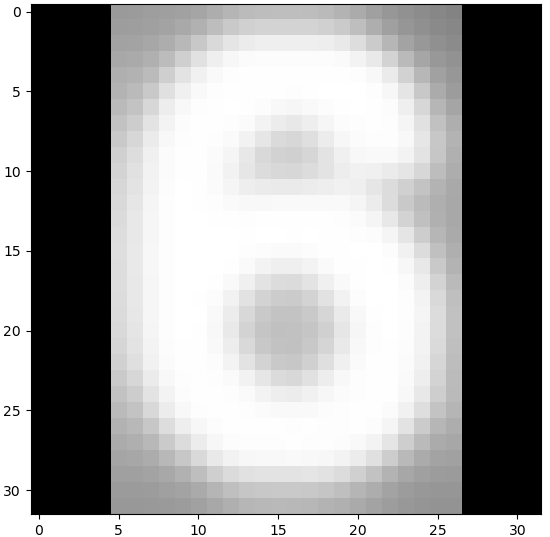
\includegraphics[height=\x1cm]{3_Reconocimiento/Figs/test_sample6_bad_padded2}
        \caption{Imagen hasta el paso 2 en condiciones no controladas.}
    \end{subfigure}
    \hfill
    \begin{subfigure}[t]{0.3\textwidth}
        \centering
        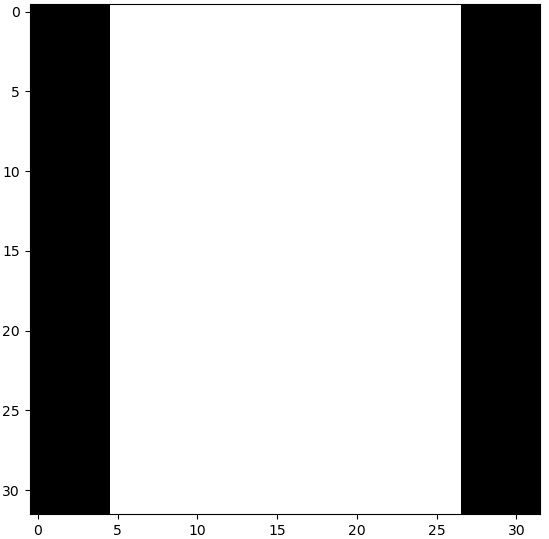
\includegraphics[height=\x1cm]{3_Reconocimiento/Figs/test_sample6_bad_otsu2}
        \caption{Imagen hasta el paso 3 en \\ condiciones no controladas.}
    \end{subfigure}
\end{figure}

La precisión del clasificador se puede medir fácilmente con una matriz de confusión, en la que directamente se identifican los falsos y verdaderos positivos.
La matriz de confusión se genera rápidamente con el código~\ref{code:confusion_matrix}.
Se armaron dos conjuntos de prueba, uno en condiciones no controladas y otro en que sí, y se probó el clasificador en ambos.
En la figura~\ref{fig:confusion_matrix_bad} se muestra la matriz de confusión para el primer conjunto (condiciones no controladas) y en la figura~\ref{fig:confusion_matrix_good} la del segundo (condiciones controladas).
\vfill
%
\begin{figure}[h!]
    \caption{Matriz de confusión del clasificador bayesiano propuesto para el conjunto de imágenes tomadas en condiciones no controladas.}
    \label{fig:confusion_matrix_bad}
    \centering
    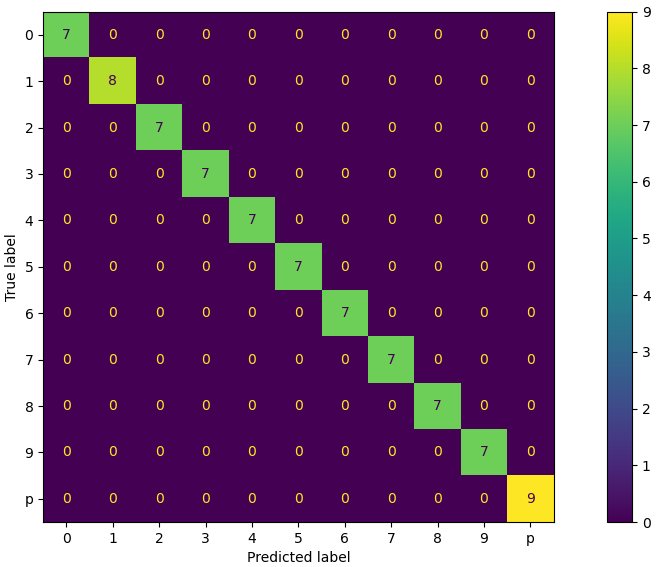
\includegraphics[width=0.5\textwidth]{3_Reconocimiento/Figs/confusion_matrix_good}
\end{figure}
%
\begin{figure}[h!]
    \caption{Matriz de confusión del clasificador bayesiano propuesto para el conjunto de imágenes tomadas en condiciones controladas.}
    \label{fig:confusion_matrix_good}
    \centering
    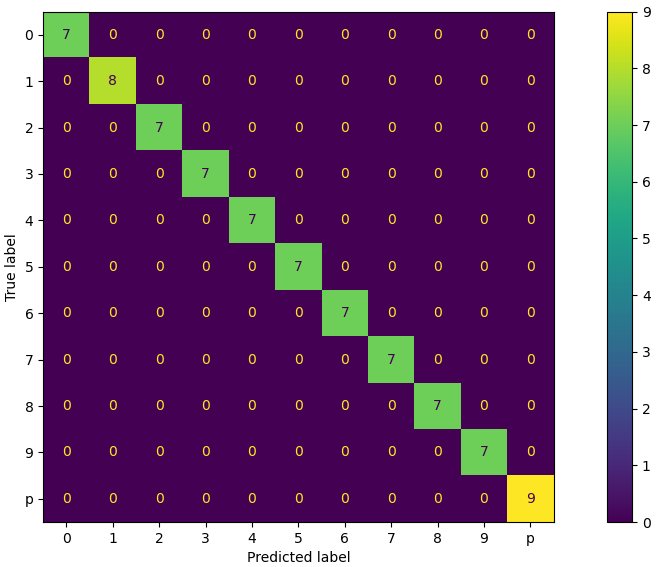
\includegraphics[width=0.5\textwidth]{3_Reconocimiento/Figs/confusion_matrix_good}
\end{figure}


\section*{Discusión}

Los resultados obtenidos demuestran un funcionamiento satisfactorio en general, tanto del procesamiento de las imágenes como del clasificador.
Aunque evidentemente es un método simplificado, resulta ser eficaz y eficiente, pues cumple con el objetivo de reconocimiento de caracteres empleando pocos recursos computacionales y cortos tiempos de entrenamiento del clasificador y del procesamiento de las imágenes, lo que permite que el método sea empleado en ordenadores con baja capacidad de procesamiento y en aplicaciones de funcionamiento en tiempo real, como se pretende en este proyecto.
Aunque el clasificador bayesiano es de las técnicas más sencillas de aprendizaje de máquina, tiene un desempeño aceptable en muchas aplicaciones reales y no requiere una base de datos de entrenamiento demasiado extensa \citepalias{Scikit-learndevelopers2022}.

Particularmente, cada una de las etapas de procesamiento resulta ser crucial en el resultado.
Por ejemplo la etapa de suavizado permite eliminar variaciones de intensidad de alta frecuencia como las irregularidades en el relleno de los dígitos debidas a la construcción de la pantalla del sonómetro, como en pantallas led, por ejemplo (cf.~\ref{fig:good_conditions_original} y~\ref{fig:good_conditions_padded}).
Sin este suavizado es posible que en la umbralización no se obtengan segmentos homogéneos que representen correctamente un dígito.
La binarización de la imagen, buscando el umbral con el método de Otsu, garantiza que se haga una discriminación correcta entre el fondo de la pantalla y el dígito, en función de la distribución de las intensidades de píxeles, esto aporta confiabilidad en la segmentación independientemente de la forma y color de los números.
Y el descriptor SIFT es bien conocido por su robustez frente a transformaciones afines o cambios en el punto de vista 3D, lo que contribuye a asegurar la eficacia en la medición de características aun cuando hay variaciones en la posición de la cámara respecto a la pantalla del sonómetro;
además, que esté basado en la dirección de los gradientes, lo hace adecuado para cuantizar de algún modo las formas de los contornos de los dígitos.

No obstante, a pesar de la eficiencia y simplicidad del clasificador bayesiano normal, lo cierto es que el resultado de clasificación es bastante sensible si se obtienen resultados erróneos en el procesamiento anterior.
Por ejemplo, por efectos de bajo contraste o desenfoques que deforman los segmentos, podría haber confusiones en la clasificación, principalmente en clases que son muy similares en sus características, como entre el $6$ y el $8$ o entre el $9$ y el $8$, pues al deformarse el segmento a causa de esos ruidos, el $6$ o el $9$ cierran el trazo faltante y se asemejan a un $8$, o alguno de los huecos se rellena y se asemejan a un $0$.
Sin embargo, en los ensayos del sistema de reconocimiento se pudo comprobar que esto ocurre cuando la posición o configuración de la cámara no es la adecuada y los efectos del desenfoque o la iluminación son más pronunciados.
Cuando las condiciones de captura de la imagen son controladas (por ejemplo, ajustando en la cámara la distancia focal y la apertura del diafragma adecuadas, limpiando la pantalla del equipo para evitar borrosidad e incluso buscando una posición apropiada del sonómetro y la cámara para mitigar las reflexiones de las fuentes de luz del lugar), la eficacia del clasificador es de un $100\%$, como se puede notar en la matriz de confusión de la figura~\ref{fig:confusion_matrix_good}.
